\documentclass{article}
\usepackage{tikz}
\usetikzlibrary{arrows.meta,positioning,calc,shapes.geometric}
\pagestyle{empty}
\begin{document}
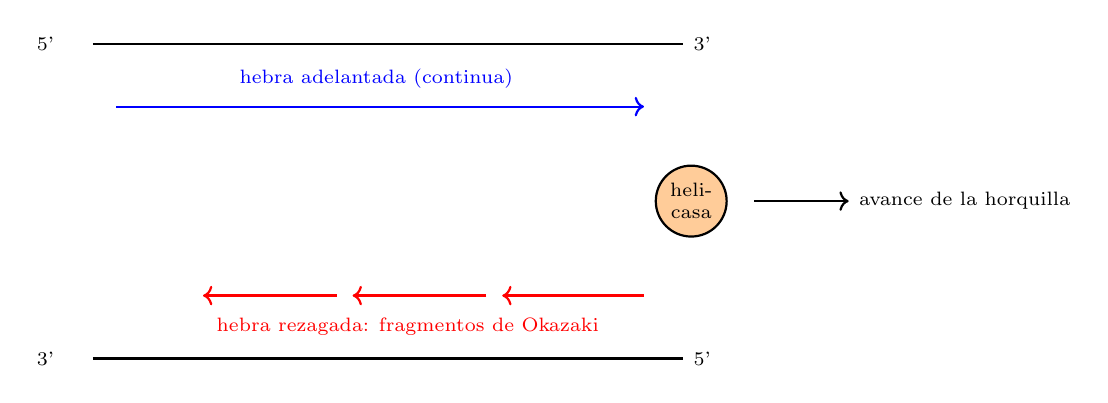
\begin{tikzpicture}
\tikzset{every node/.append style={align=center}}

\draw[thick] (0,2) -- (7.5,2) node[right, font=\scriptsize] {3'}; \draw[thick] (0,-2) -- (7.5,-2) node[right, font=\scriptsize] {5'};
\node[font=\scriptsize] at (-0.6,2) {5'}; \node[font=\scriptsize] at (-0.6,-2) {3'};
\draw[thick, fill=orange!40] (7.6,0) circle (0.45); \node[font=\scriptsize, align=center] at (7.6,0) {heli-\\casa};
\draw[->, thick, blue] (0.3,1.2) -- (7.0,1.2); \node[font=\scriptsize, blue] at (3.6,1.55) {hebra adelantada (continua)};
\foreach \x/\y in {5.2/7.0,3.3/5.0,1.4/3.1} {\draw[->, thick, red] (\y,-1.2) -- (\x,-1.2);}
\node[font=\scriptsize, red] at (4.0,-1.6) {hebra rezagada: fragmentos de Okazaki};
\draw[->, thick] (8.4,0) -- (9.6,0) node[right, font=\scriptsize] {avance de la horquilla};

\end{tikzpicture}
\end{document}
